\documentclass[a4paper,5pt]{amsbook}
%%%%%%%%%%%%%%%%%%%%%%%%%%%%%%%%%%%%%%%%%%%%%%%%%%%%%%%%%%%%%%%%%%%%%

\usepackage{booktabs}
\usepackage{graphicx}
% \usepackage[]{float}
\usepackage{amssymb}
% \usepackage{amsfonts}
% \usepackage[]{amsmath}
% \usepackage[]{epsfig}
% \usepackage[brazil]{babel}
% \usepackage[utf8]{inputenc}
% \usepackage{verbatim}
%\usepackage[]{pstricks}
%\usepackage[notcite,notref]{showkeys}
\usepackage{subcaption}
\usepackage[inline]{enumitem}

%%%%%%%%%%%%%%%%%%%%%%%%%%%%%%%%%%%%%%%%%%%%%%%%%%%%%%%%%%%%%%

\newcommand{\sen}{\text{sen}}
\newcommand{\ds}{\displaystyle}

%%%%%%%%%%%%%%%%%%%%%%%%%%%%%%%%%%%%%%%%%%%%%%%%%%%%%%%%%%%%%%%%%%%%%%%%

\setlength{\textwidth}{16cm} %\setlength{\topmargin}{-0.1cm}
\setlength{\leftmargin}{1.2cm} \setlength{\rightmargin}{1.2cm}
\setlength{\oddsidemargin}{0cm}\setlength{\evensidemargin}{0cm}

%%%%%%%%%%%%%%%%%%%%%%%%%%%%%%%%%%%%%%%%%%%%%%%%%%%%%%%%%%%%%%%%%%%%%%%%

% \renewcommand{\baselinestretch}{1.6}
% \renewcommand{\thefootnote}{\fnsymbol{footnote}}
% \renewcommand{\theequation}{\thesection.\arabic{equation}}
% \setlength{\voffset}{-50pt}
% \numberwithin{equation}{chapter}

%%%%%%%%%%%%%%%%%%%%%%%%%%%%%%%%%%%%%%%%%%%%%%%%%%%%%%%%%%%%%%%%%%%%%%%

\begin{document}
\thispagestyle{empty}
\hspace{-0.6cm}
\begin{minipage}[p]{0.14\linewidth}
	
\includegraphics[scale=0.24]{ufgd.png}
\end{minipage}
\begin{minipage}[p]{0.7\linewidth}
\begin{tabular}{c}
\toprule{}
{{\bf UNIVERSIDADE FEDERAL DA GRANDE DOURADOS}}\\
{{\bf Prof.\ Adriano Barbosa}}\\

{{\bf C\'alculo 2 --- Avalia\c{c}\~ao P1}}\\

\midrule{}
Matem\'atica\hspace{5cm}1 de Fevereiro de 2017 \\
\bottomrule{}
\end{tabular}
\vspace{-0.45cm}
%
\end{minipage}
\begin{minipage}[p]{0.15\linewidth}
\begin{flushright}
\def\arraystretch{1.2}
\begin{tabular}{|c|c|}  % chktex 44
\hline\hline  % chktex 44
1 & \hspace{1.2cm} \\
\hline  % chktex 44
2& \\
\hline  % chktex 44
3& \\
\hline  % chktex 44
4&  \\
\hline  % chktex 44
5&  \\
\hline  % chktex 44
{\small Total}&  \\
\hline\hline  % chktex 44
\end{tabular}
\end{flushright}
\end{minipage}

%------------------------
\vspace{0.5cm}
{\bf Aluno(a):}\dotfill{}  % chktex 36
%----------------------------

\vspace{0.2cm}
%%%%%%%%%%%%%%%%%%%%%%%%%%%%%%%%   formulario  inicio  %%%%%%%%%%%%%%%%%%%%%%%%%%%%%%%%
\begin{enumerate}
	\vspace{0.5cm}

	\item Determine se as afirma\c{c}\~oes abaixo s\~ao verdadeiras ou falsas.
		Justifique quando for verdadeira e d\^e um contra exemplo quando for
		falsa.
		\begin{enumerate}
			\item Se $f$ e $g$ s\~ao cont\'{\i}nuas em $[a,b]$, ent\~ao $\ds\int_a^b
				f(x)g(x)\ dx = \left(\int_a^b f(x)\ dx\right)\left(\int_a^b
					g(x)\ dx\right)$.
			\item Se $f'$ \'e cont\'{\i}nua em $[a,b]$, ent\~ao $\ds\int_a^b f'(v)\ dv =
				f(b) - f(a)$.
			\item Se $f$ \'e cont\'{\i}nua em $[a,b]$, ent\~ao
				$\ds\frac{d}{dx}\left(\int_a^b f(x)\ dx\right) = f(x)$.
			\item Se $f$ \'e cont\'{\i}nua em $[a,b]$, ent\~ao
				$\ds\frac{d}{dx}\left(\int_a^x f(t)\ dt\right) = f(x)$, $a \le
				x \le b$.
		\end{enumerate}
	\vspace{0.5cm}

	\item
		\begin{enumerate}
			\item Calcule a integral $\ds\int_0^2 (x^2 - x)\ dx$ pela
				defini\c{c}\~ao.
			\item Use o Teorema Fundamental do C\'alculo para verificar sua
				resposta.
		\end{enumerate}
	\vspace{0.5cm}

	\item Calcule as \'areas abaixo:

		\begin{enumerate*}
			\item 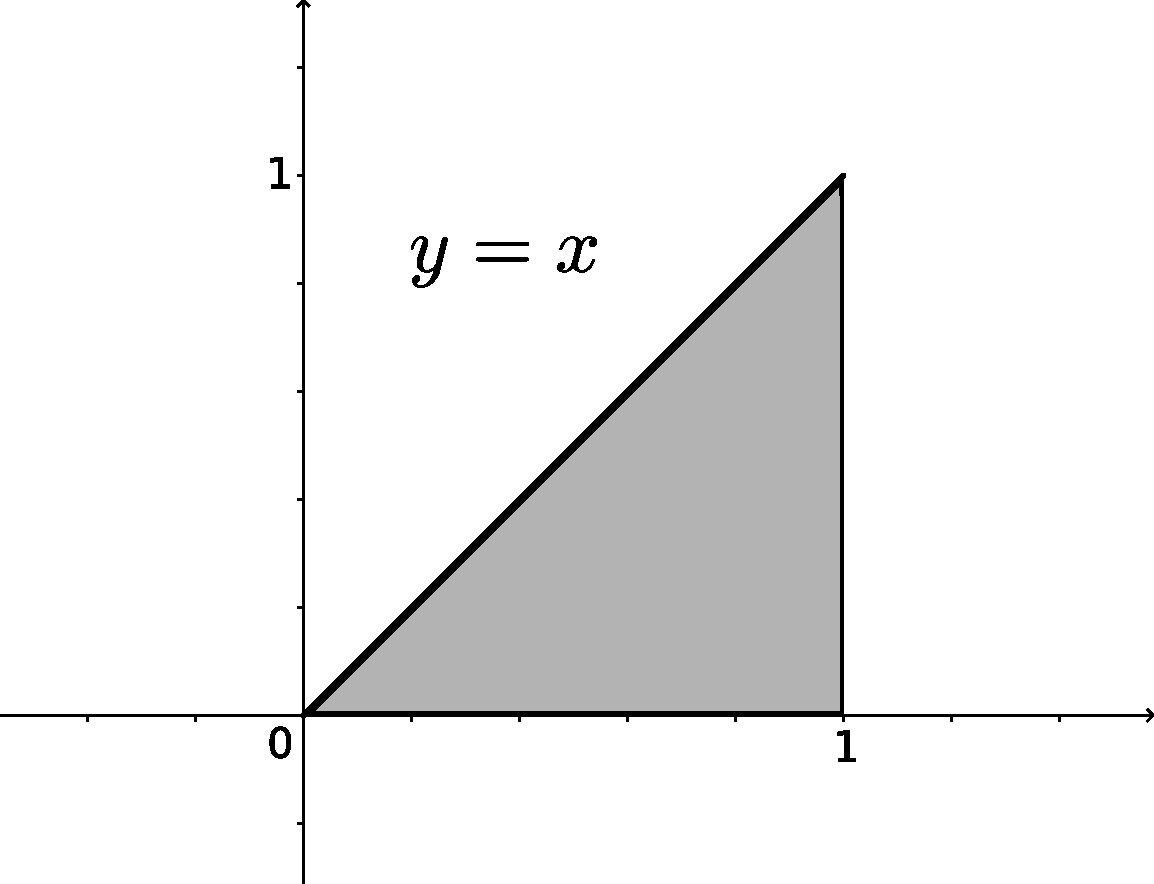
\includegraphics[width=0.25\textwidth]{3a.pdf}
			\item 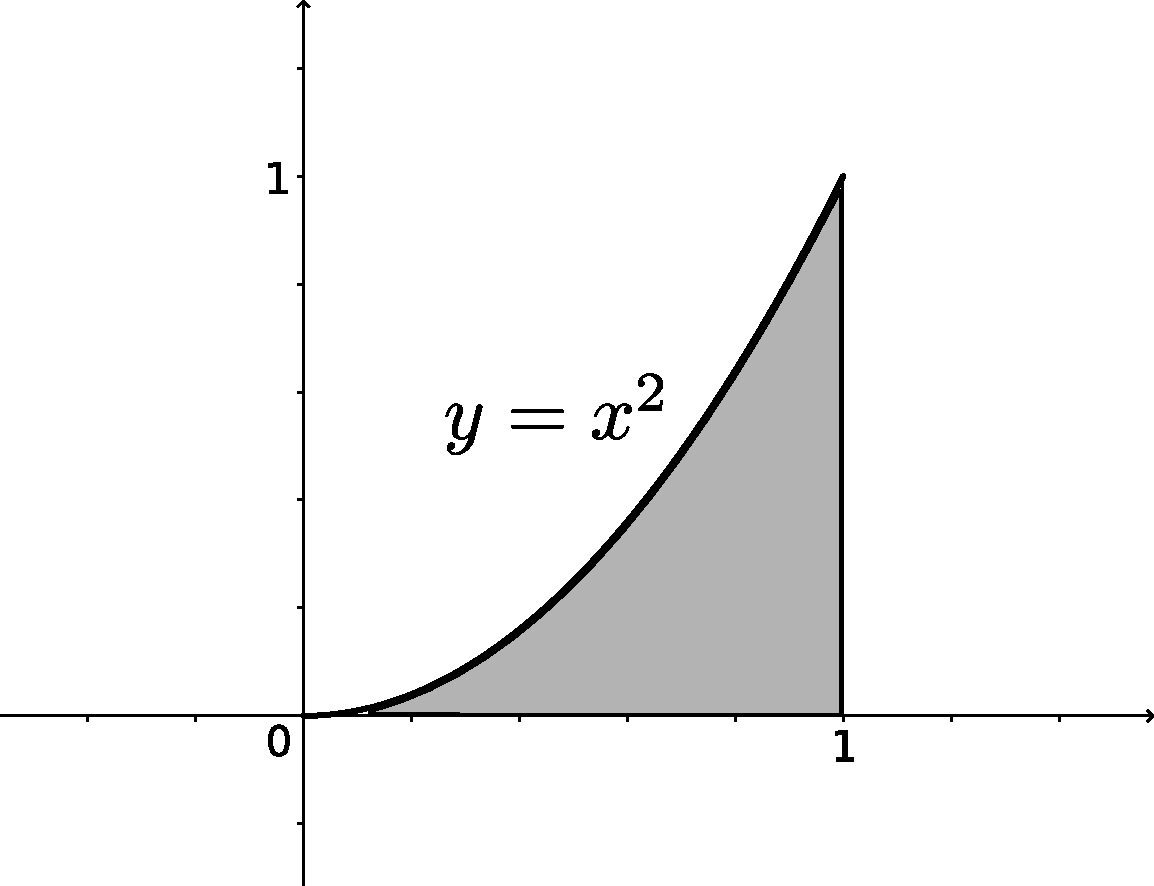
\includegraphics[width=0.25\textwidth]{3b.pdf}
			\item 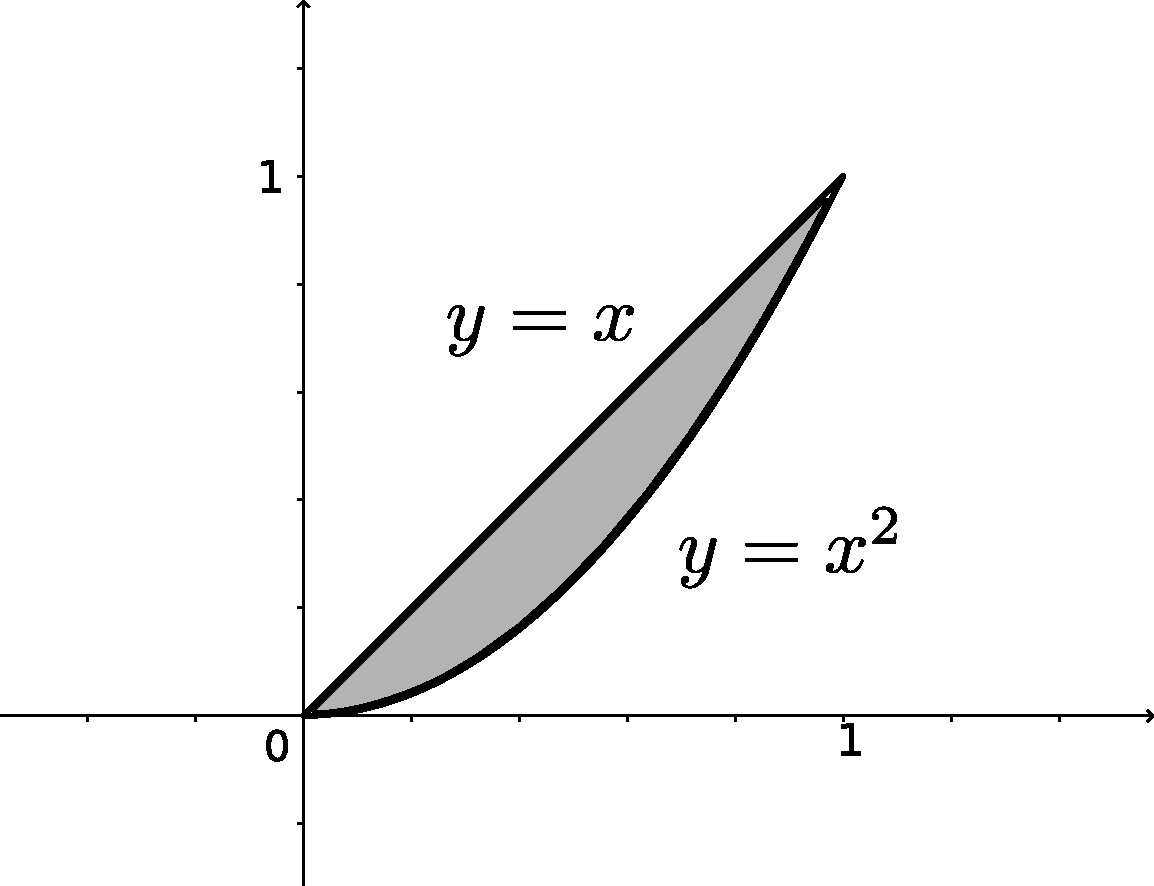
\includegraphics[width=0.25\textwidth]{3c.pdf}
		\end{enumerate*}
	\vspace{0.5cm}

	\item Calcule a intergarl definida $\ds\int_0^4 \frac{x}{\sqrt{1+2x}}\ dx$.
	\vspace{0.5cm}

	\item Calcule a integral indefinida $\ds\int x e^{-2x}\ dx$.
\end{enumerate}

\vspace{0.5cm}
F\'ormulas \'uteis:

$\ds\sum_{i=1}^n i = \frac{n(n+1)}{2}$\hspace{2cm}
$\ds\sum_{i=1}^n i^2 = \frac{n(n+1)(2n+1)}{6}$\hspace{2cm}
$\ds\sum_{i=1}^n i^3 = {\left[\frac{n(n+1)}{2}\right]}^2$

\begin{flushright}
	\vspace{1cm}
	\textit{Boa Prova!}
\end{flushright}

\end{document}
